\documentclass[10pt,twocolumn,a4paper]{extarticle}
\usepackage{iftex}
\ifPDFTeX
  \usepackage[T1]{fontenc}\usepackage[utf8]{inputenc}\usepackage{lmodern}
\else
  \usepackage{fontspec}
\fi
\usepackage{microtype,float}
\usepackage[a4paper,margin=1.45cm,columnsep=0.6cm]{geometry}
\usepackage{amsmath,amssymb,bm,booktabs,graphicx,enumitem,titlesec,xcolor,caption}
\setlist[itemize]{nosep,leftmargin=1.1em,label=\textbullet}
\titleformat{\section}{\normalsize\bfseries\sffamily}{\thesection}{0.5em}{}
\titlespacing*{\section}{0pt}{6pt}{2pt}
\captionsetup{font=footnotesize,labelfont=bf,skip=3pt}
\setlength{\parskip}{2pt}\setlength{\parindent}{0pt}
\setlength{\abovedisplayskip}{3pt}\setlength{\belowdisplayskip}{3pt}
\setlength{\abovedisplayshortskip}{2pt}\setlength{\belowdisplayshortskip}{2pt}
\setlength{\textfloatsep}{6pt}\setlength{\dbltextfloatsep}{6pt}\setlength{\floatsep}{5pt}
\newcommand{\code}[1]{\texttt{\small #1}}
\pagestyle{empty}

\begin{document}
\twocolumn[{%
\begin{center}
{\Large\bfseries\sffamily A Systematic Multi-Asset Strategy: From Data to Backtest}\\[3pt]
{\small Jean Philippe N'Dri \quad\textbullet\quad 6 October 2026 \quad\textbullet\quad code: \code{multiasset-strat}, built on \code{portopt}}
\end{center}
\vspace{-2pt}
\noindent\small\textbf{Abstract.} Each month the strategy selects 10 lines out of 132 assets (US stocks, ETFs, bonds, commodities) using price signals, weights them by risk budgeting, and limits rotations to account for a fixed fee per order. Over 2018--2026, a period not used to choose the signals, the net Sharpe ratio is 1.15 against 0.82 for a 60/40 portfolio. This result is overstated by an uncorrected survivorship bias.
\vspace{6pt}
}]

\section{Data and universe}
Adjusted closing prices (dividends reinvested) come from Yahoo Finance from 2008 onwards and are converted into daily simple returns $r_{i,t}=P_{i,t}/P_{i,t-1}-1$. The universe has four sleeves and one safe asset:
\begin{itemize}
\item \textbf{Stocks} (96): large caps from the S\&P~500 and the Nasdaq~100;
\item \textbf{ETFs} (21): indices, factors, themes, multi-asset;
\item \textbf{Bonds} (8) and \textbf{commodities} (7);
\item \textbf{Cash}: \code{SHY}, which receives the capital of empty slots.
\end{itemize}
An asset is eligible at date $t$ only if it has 252 consecutive returns before $t$, so late listings enter the universe naturally. The ETFs are US proxies; live execution goes through UCITS equivalents.

\section{Signals}
All signals are computed on the window $[t-252,\,t)$, with no information after $t$. Thirteen price signals taken from the literature were tested one by one, per sleeve, on 2009--2017, then checked once on 2018--2026. Five are kept.

\textbf{Trend} (stocks, ETFs, commodities):
\begin{align*}
\text{mom}_{12\text{-}1} &= \frac{P_{t-21}}{P_{t-252}}-1, &
\text{mom}_{6\text{-}1} &= \frac{P_{t-21}}{P_{t-126}}-1,\\
\text{ma}_{200} &= \frac{P_t}{\mathrm{SMA}_{200}}-1, &
\text{ma}_{50/200} &= \frac{\mathrm{SMA}_{50}}{\mathrm{SMA}_{200}}-1.
\end{align*}
\textbf{Mean reversion} (bonds):
\[
\text{boll}_{20} = -\,\frac{P_t-\mathrm{SMA}_{20}}{\sigma_{20}(P)}.
\]
Each signal $x_{i,k}$ is winsorised at 1\%/99\% and standardised \emph{within its sleeve} $g$; the score is the average of the sleeve's $K_g$ signals:
\[
z_{i,k}=\frac{x_{i,k}-\mu^{(g)}_k}{\sigma^{(g)}_k},\qquad S_i=\frac{1}{K_g}\sum_{k=1}^{K_g} z_{i,k}.
\]
Standardising per sleeve avoids comparing the momentum of a stock with that of a bond, whose dispersions have nothing in common. An \textbf{absolute filter} is added: an asset can be bought only if $P_t>\mathrm{SMA}_{200}$.

Low volatility, part of the first version of the score, was removed: its information coefficient is negative for stocks and ETFs in both sub-periods.

\section{Selection}
The portfolio holds 5 stocks, 2 ETFs, 2 bonds and 1 commodity. In each sleeve the best scores are picked among the assets passing the filter. Three rules limit rotations:
\begin{itemize}
\item \textbf{hysteresis}: a held line leaves only if it breaks its trend or drops out of the top 40\% of its sleeve;
\item \textbf{at most two exits} per rebalancing, broken trends first;
\item a slot with no candidate is parked in \code{SHY}.
\end{itemize}

\section{Allocation}
The weights of the $n$ selected lines solve a risk budgeting problem. With $\bm\Sigma$ the Ledoit--Wolf covariance estimated on the window, the relative contribution of line $i$ is
\[
\mathrm{RC}_i=\frac{w_i\,(\bm\Sigma\bm w)_i}{\bm w^{\top}\bm\Sigma\bm w},\qquad \sum_i \mathrm{RC}_i=1,
\]
and we impose $\mathrm{RC}_i=b_i$, where the sleeve budgets are 40\% for stocks, 24\% for ETFs, 24\% for bonds and 12\% for commodities, split equally between the lines of a sleeve. The solution is obtained by coordinate descent on Spinu's convex formulation,
\[
\bm y^{\star}=\arg\min_{\bm y>0}\ \tfrac12\,\bm y^{\top}\bm\Sigma\bm y-\sum_i b_i\ln y_i,\qquad \bm w=\frac{\bm y^{\star}}{\bm 1^{\top}\bm y^{\star}}.
\]
Weights are then bounded ($5\%\le w_i\le 20\%$, with a 3\% floor for a stock). Since these bounds distort the budgets, the stock budget is re-imposed as a ceiling by bisection on a scaling factor applied to the sleeve.

\section{Turnover constraints}
Let $\bm w^{-}$ be the portfolio held (drifted weights) and $\bm w^{\star}$ the target. Because fees are fixed per order, cost depends on the \emph{number} of orders, not on the amount traded. Execution therefore applies:
\begin{itemize}
\item a \textbf{no-trade band}: no order if $|w^{\star}_i-w^{-}_i|<2$ points;
\item a \textbf{cap} $\tau_t=\sum_i|w_{i,t}-w^{-}_{i,t}|\le 40\%$, giving up the smallest adjustments first.
\end{itemize}
Weight bounds take precedence over the cap, which stays soft for the last rotation.

\begin{figure*}[t]
\centering
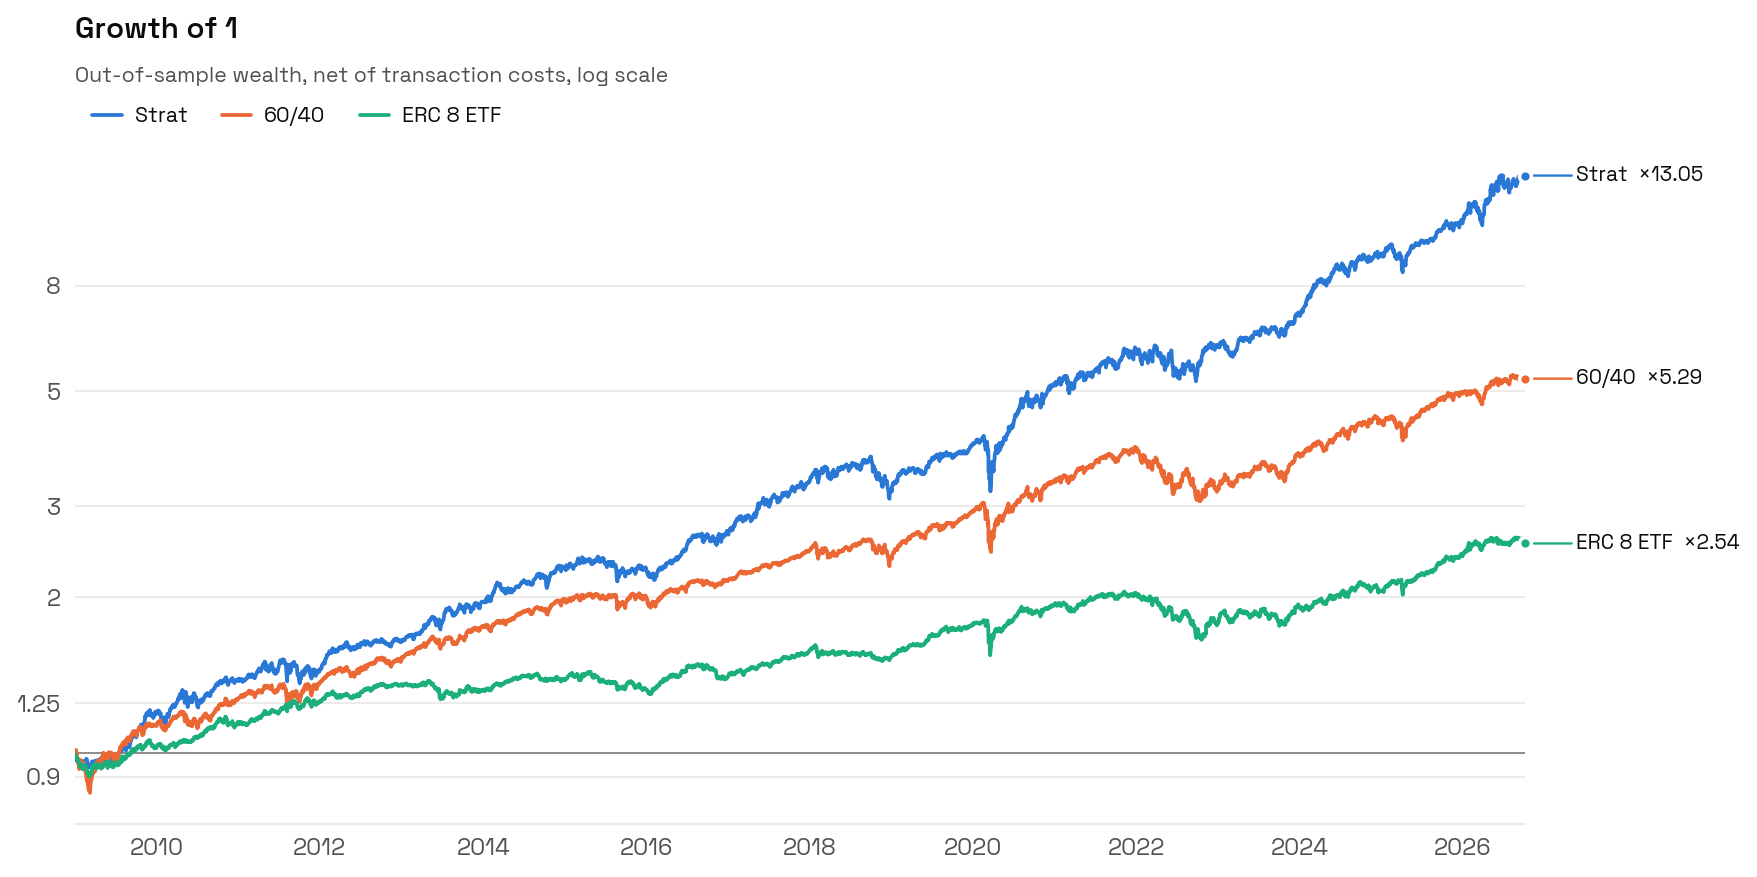
\includegraphics[width=0.8\textwidth]{wealth.png}
\caption{Growth of 1 invested, net of fees, log scale.}
\end{figure*}

\section{Backtest}
The backtest is walk-forward: at each date $t$ of the grid (every 21 trading days), weights are computed on $r_{[t-252,\,t)}$ and applied from $r_t$ onwards, then drift freely until the next rebalancing. The cost paid at $t$ is
\[
c_t=s\,\tau_t+\frac{f\,n^{\text{orders}}_t}{\mathrm{NAV}_t},
\]
with $s=5$~bps, $f=1$~EUR per order and $\mathrm{NAV}_0=10{,}317$~EUR. A fixed fee therefore weighs more on a small account. Two benchmarks bear the same fees: a 60/40 (\code{SPY}/\code{IEF}) and a risk parity on 8 ETFs with no signal.

\section{Results}
\begin{table}[H]
\centering\footnotesize
\begin{tabular}{@{}lrrr@{}}
\toprule
Net of fees & Strategy & 60/40 & ERC 8 ETFs\\
\midrule
\multicolumn{4}{@{}l}{\emph{2009--2026}}\\
Annualised return & 15.6\% & 9.9\% & 5.4\%\\
Volatility & 12.4\% & 10.3\% & 7.2\%\\
Sharpe & 1.23 & 0.96 & 0.76\\
Maximum drawdown & $-21.9\%$ & $-21.5\%$ & $-19.4\%$\\
\midrule
\multicolumn{4}{@{}l}{\emph{2018--2026, out of sample}}\\
Annualised return & 16.9\% & 9.2\% & 5.6\%\\
Volatility & 14.5\% & 11.5\% & 8.1\%\\
Sharpe & 1.15 & 0.82 & 0.71\\
\bottomrule
\end{tabular}
\caption{Performance net of fees. Signals were chosen on 2009--2017.}
\end{table}
Over 2018--2026, the gap with the 60/40 is 7.2 points per year ($t=2.4$). The strategy sends 4.3 orders per rebalancing on average, for 0.4\% of annual fees and a turnover of 387\% per year.

\textbf{Risk checks.} The portfolio never exceeds 10 lines or 21.7\% per line. The stock sleeve carries 44\% of risk on average (target 40\%, maximum 59\% between two rebalancings). Ex-ante variance splits into 62\% market beta and 26\% specific risk, of which 12\% comes from stocks. The worst daily loss caused by a single line is 2.3 NAV points. The turnover cap is exceeded in 16.5\% of rebalancings.

\section{Limitations}
\begin{itemize}
\item \textbf{Survivorship bias.} The stocks are today's large caps. A trend signal applied to survivors is flattered, by an amount that has not been quantified.
\item \textbf{Weak statistical evidence.} No single signal survives the Benjamini--Hochberg correction over the 52 tests (best $q$-value: 0.46). The effect on stocks lives in the tail: the top~5 outperforms while the rank IC is zero.
\item \textbf{Sector concentration.} There is no sector constraint: on 5 October 2026, the five selected stocks are all semiconductors.
\item \textbf{Currency.} The backtest is in dollars, with no EUR/USD effect.
\end{itemize}
\end{document}
